\subsection{Parity Symbol and Sequence Number}
To deal with the unsynchronized problem, we add additional schemes.
The sequence number is used to identify any missing symbol or redundant symbol. Missing symbols will be reconstructed with corresponding parity symbols, while redundant symbols with the same sequence number will be dropped.

As symbols could be lost or corrupted due to the time gap of the channel or if the exposure time is an integer multiple of the signal period,
a parity symbol is inserted for every $n$ data symbols by \textbf{XOR-ing} all $n$ data symbols, so that if only one of the $n$ data symbols or the parity symbol is not correctly received, the receiver can \textbf{recover the lost symbol}. The number of parity symbols that should be added to a packet can be determined by calculating expected number of lost symbols in a packet using the probability equation in \autoref{sec:unsync}. 

After constructing a sequence of symbols, including the parity symbol, to be transmitted, we label each symbol with a \textbf{1.5 bit} sequence number $=\{0,1,2\}$.
The sequence number can be obtained by calculating the index number modulo 3.
The sequence number is then combined with the data symbol to become one meta symbol, then mapped to one of the selected signal periods.
Note that the sequence number reduces the number of bits that can be represented by each symbol by 1.5 bits. However, this is required to detect \textbf{lost symbols} (when the transmitting frame duration is smaller than the receiving frame duration) or \textbf{redundant symbols} (when the transmitting frame duration is larger than the receiving frame duration).
Taking the assumption into consideration, it can be proved that there could be no consecutive symbol losses. Thus, a 1.5 bit sequence number, $\{0,1,2\}$, would be sufficient determine the location of a lost symbol in the sequence. 
% Note that the sequence number will be represented by the most significant 1.5 bits in a symbol, i.e., symbols with different sequence numbers will be separated with a large margin, and thus getting an erroneous sequence number is unlikely. \\
% The sequence number is used to identify any missing symbol or redundant symbol. Missing symbols will be reconstructed with corresponding parity symbols, while redundant symbols with the same sequence number will be dropped. In the case that redundant symbols with the same sequence number is demodulated to different symbols, the one decoded with the largest image area will be used.

\begin{figure}[!t] %move forward
  %\centering
  \hspace{-1em}
  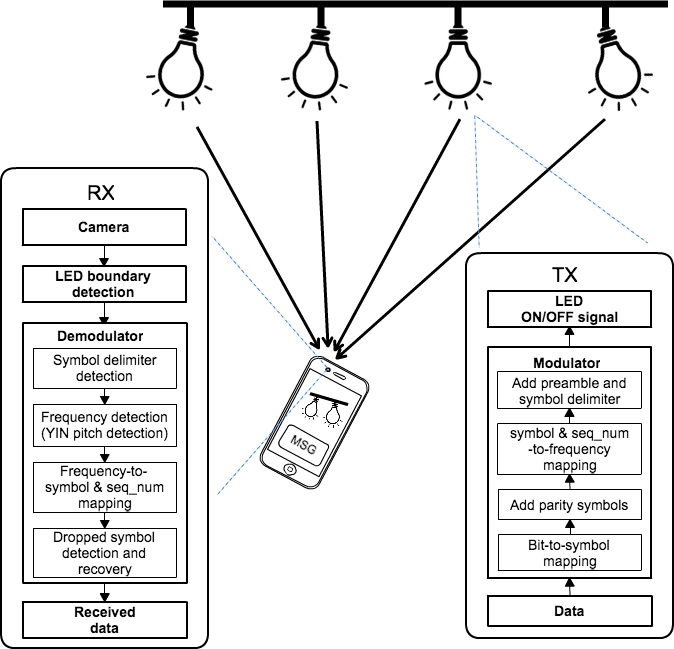
\includegraphics[scale=0.375]{pic/arch.png} 
  \caption{System Architecture of RollingLight}
  \label{fig:SystemArchitecture}
\end{figure}

\subsection{Preamble Symbol} 
The preamble symbol, which has a signal period known to the receiver, is inserted at the beginning of the symbol sequence.
The preamble symbol serves two functions: one is for the receiver to detect the start of the packet and start the subsequent demodulation process, while the other is for the receiver to accurately \textbf{calibrate its $T_r$ value} based on the period estimate of the preamble, so that the error of the period estimates of all subsequent symbols in this packet can be minimized. As a result, the signal period with the smallest error variation is selected as the period for the preamble symbol. %In our experiment, we select the 5657.3886 Hz as the period for the preamble symbol. This is the highest frequency used in our design. 

\subsection{Symbol Delimiter}
% Finally, another signal period is selected as the symbol delimiter signal period.
This scheme is also for addressing the unsynchronized issue.
We select another signal period as the symbol delimiter.
In order to easily \textbf{separate consecutive symbols} in the same image, i.e., two areas in the image showing signals with different periods, a signal with this signal period will be transmitted for a short duration between any two symbol transmissions as \autoref{fig:FD} shows. 

\begin{figure}[!t]
  \centering
  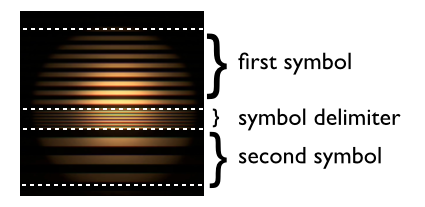
\includegraphics[scale=0.4]{pic/symbol_delimiter.png} 
  \caption{Symbol delimiter illustration.}
  \label{fig:FD}
\end{figure}

\begin{figure*}[!t]
   \centering
   \begin{subfigure}[h]{0.16\textwidth}
      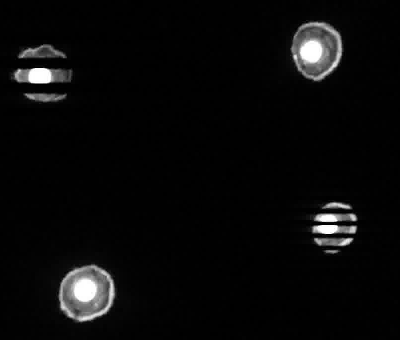
\includegraphics[width=\textwidth]{pic/bbox/bbox_A_original_crop.png}
      \caption{Original} \label{fig:bbox_ori}
   \end{subfigure}%
   ~
   \begin{subfigure}[h]{0.16\textwidth}
      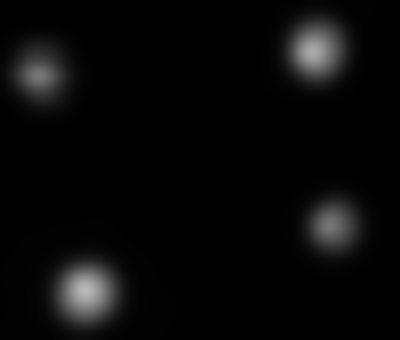
\includegraphics[width=\textwidth]{pic/bbox/bbox_B_gaussianBlur_crop.png}
      \caption{Gaussian Blur} \label{fig:bbox_blur}
   \end{subfigure}%
   ~  
   \begin{subfigure}[h]{0.16\textwidth}
      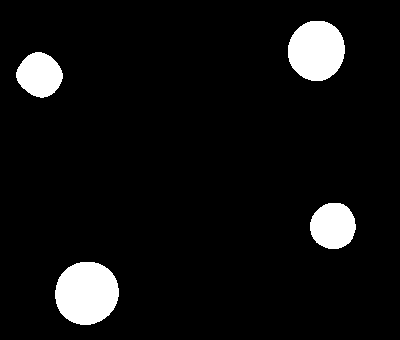
\includegraphics[width=\textwidth]{pic/bbox/bbox_C_OTSU_crop.png}
      \caption{Binary OTSU} \label{fig:bbox_otsu}
   \end{subfigure}%
   ~
   \begin{subfigure}[h]{0.16\textwidth}
      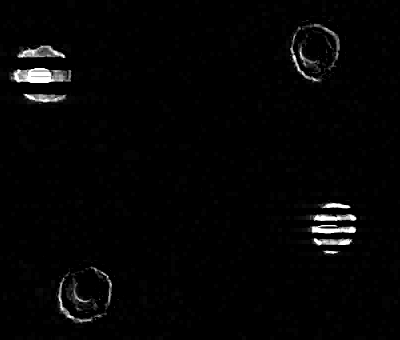
\includegraphics[width=\textwidth]{pic/bbox/bbox_E_template_crop.png}
      \caption{Template} \label{fig:bbox_template}
   \end{subfigure}%
   ~
   \begin{subfigure}[h]{0.16\textwidth}
      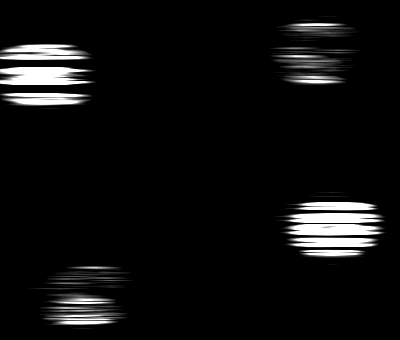
\includegraphics[width=\textwidth]{pic/bbox/bbox_F_haar_crop.png}
      \caption{Haar-like Feature} \label{fig:bbox_haar}
   \end{subfigure}%
   ~   
   \begin{subfigure}[h]{0.16\textwidth}
      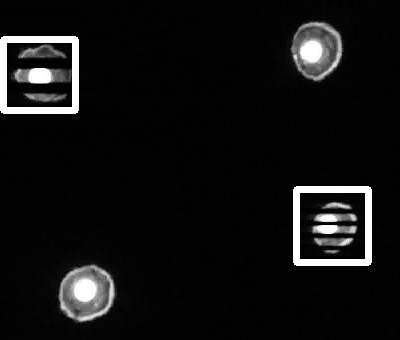
\includegraphics[width=\textwidth]{pic/bbox/bbox_H_stripedLED_crop.png}
      \caption{Result} \label{fig:bbox_result}
   \end{subfigure}%
   \\
   \begin{subfigure}[h]{0.16\textwidth}
      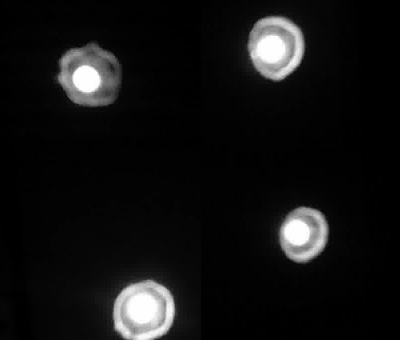
\includegraphics[width=\textwidth]{pic/bbox/bbox_A_original400_crop.png}
      \caption{Original} \label{fig:bbox_ori}
   \end{subfigure}%
   ~
   \begin{subfigure}[h]{0.16\textwidth}
      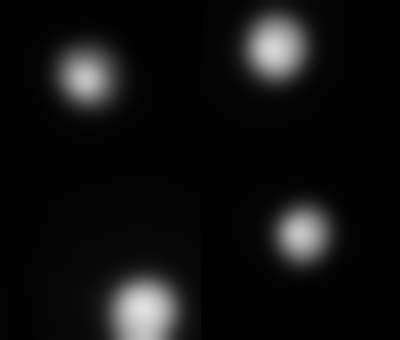
\includegraphics[width=\textwidth]{pic/bbox/bbox_B_gaussianBlur400_crop.png}
      \caption{Gaussian Blur} \label{fig:bbox_blur}
   \end{subfigure}%
   ~  
   \begin{subfigure}[h]{0.16\textwidth}
      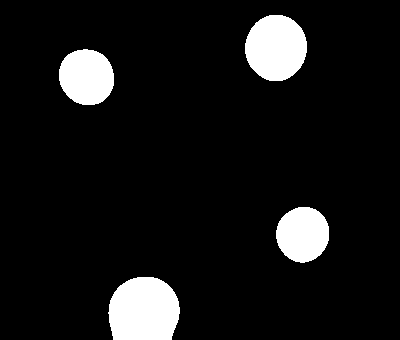
\includegraphics[width=\textwidth]{pic/bbox/bbox_C_OTSU400_crop.png}
      \caption{Binary OTSU} \label{fig:bbox_otsu}
   \end{subfigure}%
   ~
   \begin{subfigure}[h]{0.16\textwidth}
      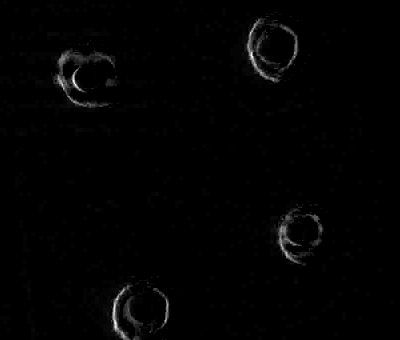
\includegraphics[width=\textwidth]{pic/bbox/bbox_E_template400_crop.png}
      \caption{Template} \label{fig:bbox_template}
   \end{subfigure}%
   ~
   \begin{subfigure}[h]{0.16\textwidth}
      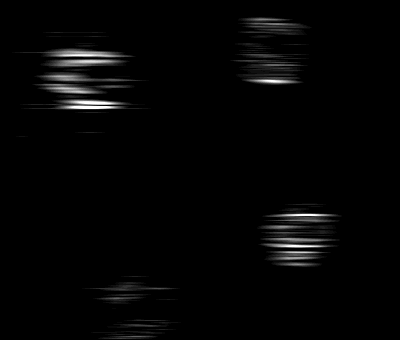
\includegraphics[width=\textwidth]{pic/bbox/bbox_F_haar400_crop.png}
      \caption{Haar-like Feature} \label{fig:bbox_haar}
   \end{subfigure}%
   ~   
   \begin{subfigure}[h]{0.16\textwidth}
      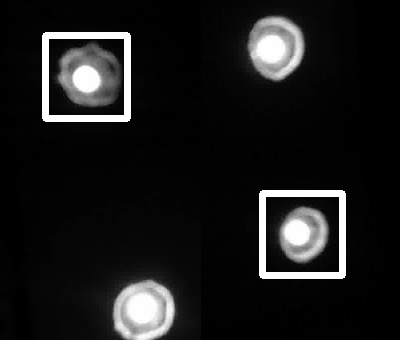
\includegraphics[width=\textwidth]{pic/bbox/bbox_H_stripedLED400_crop.png}
      \caption{Result} \label{fig:bbox_result}
   \end{subfigure}%
   \caption{LED boundary detection step-by-step. The top row of images taken with exposure duration 1/5000 sec. The bottom row of images taken with exposure time 1/400 sec. The result image detects the light with strips.}
   \label{fig:bbox}
\end{figure*}

The detection step is done by calculating the value of the difference function described in \autoref{sec:demodulation} for all possible symbol delimiter locations in the image, but only with a fixed shift value that equals the the signal period of the symbol delimiter. If the minimum value of the function for all possible delimiter locations is larger than a pre-defined threshold, then it will output the location of the symbol delimiter.

\subsection{LED Boundary Detection}
To decode the lights, the first step is to find the boundary of each light in the received image.We follow the~\cite{luxapose} to detect the lights individually. We slightly modified the detection process. To detect the light taken with larger exposure duration, we need to eliminate the background noise. Our method is maintain a buffer with latest few images, for the current image, we make a template by averaging all images in the buffer. Then we subtract the template from the current image to eliminate the noise. Another modification is the haar-like feature. Since there would be some other light in the image, we want to further detect the modulated light, that is, the light with strips. Thus the haar-like feature is added to filter the light with strips.

~\autoref{fig:bbox} shows the light detection process step-by-step. There are four lights, two of them (the top-left and the bottom-right one) are modulated. We test the detection method with two exposure time settings: the larger one 1/400 sec and the smaller one 1/5000 sec.
More sophisticated detection and tracking algorithms based on computer vision techniques can be utilized if necessary.

% \textbf{Bit-to-symbol mapping.} Data bits to be transmitted will first be split into bit patterns of a constant length. Each bit pattern is then mapped to a data symbol. \\

% \textbf{Parity symbol.} As symbols could be lost or corrupted due to the time gap of the channel or if the exposure time is an integer multiple of the signal period,
% a parity symbol is inserted for every $n$ data symbols by \textbf{XOR-ing} all $n$ data symbols, so that if only one of the $n$ data symbols or the parity symbol is not correctly received, the receiver can \textbf{recover the lost symbol}. The number of parity symbols that should be added to a packet can be determined by calculating expected number of lost symbols in a packet using the probability equation in \autoref{sec:unsync}. \\ 

% \textbf{Sequence number.} After constructing a sequence of symbols, including the parity symbol, to be transmitted, we label each symbol with a \textbf{1.5 bit} sequence number $=\{0,1,2\}$.
% The sequence number can be obtained by calculating the index number modulo 3.
% The sequence number is then combined with the data symbol to become one meta symbol, then mapped to one of the selected signal periods.
% Note that the sequence number reduces the number of bits that can be represented by each symbol by 1.5 bits. However, this is required to detect \textbf{lost symbols} (when the transmitting frame duration is smaller than the receiving frame duration) or \textbf{redundant symbols} (when the transmitting frame duration is larger than the receiving frame duration).
% Taking the assumption into consideration, it can be proved that there could be no consecutive symbol losses. Thus, a 1.5 bit sequence number, $\{0,1,2\}$, would be sufficient determine the location of a lost symbol in the sequence. 
% Note that the sequence number will be represented by the most significant 1.5 bits in a symbol, i.e., symbols with different sequence numbers will be separated with a large margin, and thus getting an erroneous sequence number is unlikely. \\

% \textbf{Preamble symbol.} Next, the preamble symbol, which has a signal period known to the receiver, is inserted at the beginning of the symbol sequence.
% The preamble symbol serves two functions: one is for the receiver to detect the start of the packet and start the subsequent demodulation process, while the other is for the receiver to accurately \textbf{calibrate its $T_r$ value} based on the period estimate of the preamble, so that the error of the period estimates of all subsequent symbols in this packet can be minimized. As a result, the signal period with the smallest error variation is selected as the period for the preamble symbol. In our experiment, we select the 5657.3886 Hz as the period for the preamble symbol. This is the highest frequency used in our design. \\

% \textbf{Symbol delimiter.} Finally, another signal period is selected as the symbol delimiter signal period.
% In order to easily \textbf{separate consecutive symbols} in the same image, i.e., two areas in the image showing signals with different periods, a signal with this signal period will be transmitted for a short duration between any two symbol transmissions. %as Figure~\ref{fig:FD} shows. 
% The transmitting light is then driven to transmit a sequence of square waves according to pre-determined list of signal periods representing the entire data packet. \\

% \begin{figure}[!t]
%   \centering
%   \includegraphics[scale=0.8]{fig/fd.png} 
%   \caption{Frame delimiter illustration. The upper shows the frame without frame delimiter; the lower shows the frame with frame delimiter.}
%   \label{fig:FD}
% \end{figure}

% \begin{figure}[!t]
%   \centering
%   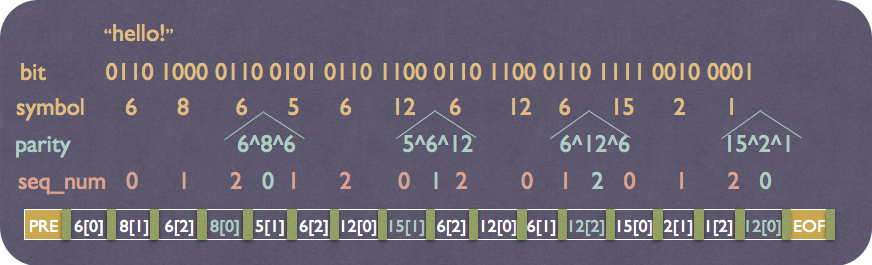
\includegraphics[scale=0.25]{fig/flow_tx.png} 
%   \caption{An example flow of the transmitter end.}
%   \label{fig:flow_tx}
% \end{figure}

% \autoref{fig:flow_tx} shows an example flow of the transmitter end. The message "hello!" is converted to the bit string, Then every 4-bit is mapped to a symbol. Assume the $P_{miss}$ is 0.25, which means a parity symbol is inserted for every 3 symbols. Next step we tag the symbols (including parity symbol) in the order of $\{0,1,2\}$ as the sequence number. The last step is to add the preamble symbol and the EOF symbol (the yellow part in the figure) at the beginning and the end of the data, and the symbol delimiter symbol (the green part in the figure) between each data symbols. 

% \textbf{LED boudary detection.} The receiving camera captures a series of images with the transmitting light. The receiver starts the demodulation process by determining the image area occupied by the transmitting light. In our system, this is done by extracting an area with very high intensity values. More sophisticated detection and tracking algorithms based on computer vision techniques can be utilized if necessary. \\

% \textbf{Symbol delimiter detection.}
% A symbol delimiter detector is then executed to determine whether a symbol delimiter area presents in the image. 
% % \autoref{fig:flow_rx} shows the received image which contains a symbol delimiter. 
% The detection step is done by calculating the value of the difference function described in \autoref{sec:demodulation} for all possible symbol delimiter locations in the image, but only with a fixed shift value that equals the the signal period of the symbol delimiter. If the minimum value of the function for all possible delimiter locations is larger than a pre-defined threshold, then it will output the location of the symbol delimiter. Then, the period detection algorithm can be executed to determine the signal periods of two image areas separated by the symbol delimiter. In this case, the signal periods of both symbols can be accurately estimated.

% % \begin{figure}[!t]
% %   \centering
% %   \includegraphics[scale=0.25]{fig/FD_illustration} 
% %   \caption{Received frame with frame delimiter.}
% %   \label{fig:FD_photo}
% % \end{figure}
% % \begin{figure}[!t]
% %   \centering
% %   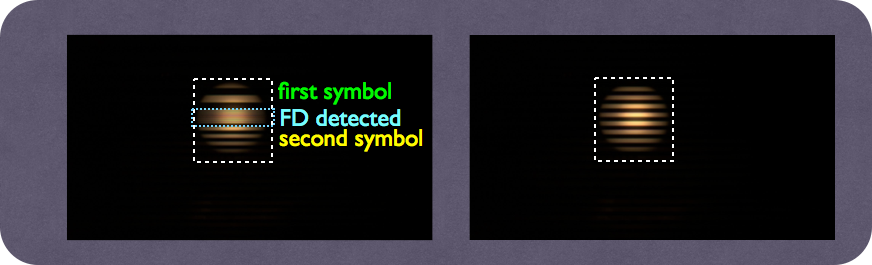
\includegraphics[scale=0.25]{fig/flow_rx.png} 
% %   \caption{An example flow of the symbol delimiter detection of the receiver end.}
% %   \label{fig:flow_rx}
% % \end{figure}

% The estimated signal period will be mapped to a meta symbol. The meta symbol is then split into a sequence number and a data symbol. \\

% \textbf{Dropped symbol detection and recovery.}
% Then, the sequence number is used to identify any missing symbol or redundant symbol. Missing symbols will be reconstructed with corresponding parity symbols, while redundant symbols with the same sequence number will be dropped. In the case that redundant symbols with the same sequence number is demodulated to different symbols, the one decoded with the largest image area will be used.

% The data string is finally obtained after mapping the sequence of data symbols back to the bit patterns, forming the original bit stream.
